\documentclass{article}
\usepackage{import}
\subimport{../}{preamble}
\begin{document}

\section{Mechanical Design}

To measure the physical properties of nanostructures on the sub-nm scale in ambient conditions is a difficult challenge. For a microscope to be capable of such measurements requires many careful considerations, the result of which is a compact experimental platform resistant to both vibrations and thermal effects.

\begin{figure}[tb]
\centering
\includegraphics[clip=true, trim=15 10 0 0]{figures/microscope_stage_design}
\caption[Mechanical design of the microscope]{\textbf{Mechanical design of the microscope}. The main features of the inverted microscopy platform are highlighted, including two independent nanopositioners, one with piezo control, situated on a removable breadboard plate above the focus of an objective. Breadboard holes enable the mounting of optomechanics close to the sample. The top plate features a sealed lid with gas inlets for environmental control.}
\label{fig:mechanical_design}
\end{figure}

The most important parts of any microscope are the sample stage and objective lens. For stable optical measurements these have to be locked together {\color{red}(mechanically referenced)} in a symmetric configuration to prevent drift, mechanical or thermal, between the sample and the focal spot. An inverted microscope design provides the best stability and the microscope platform (\figurename~\ref{fig:mechanical_design}) is designed based on this concept.
% Mechanical drift prevention:  reference points
Mechanical drift is prevented by maintaining a close reference point between the sample and the objective. In this case the sample stage is pocketed into a top plate from which the objective is screwed so that any vibrations between sample and objective occur in phase.
% Thermal drift: symmetry, coefficients of thermal expansion
Thermal drift is prevented by exploiting symmetry such that any expansion is around the objective and that all mechanical plates expand at the same rate. Cast aluminium is also used for plate construction for its lower coefficient of thermal expansion compared to aluminium, whilst still remaining cheap and easily machinable compared with steel or titanium.
% Further stability
The overall microscope platform is constructed \SI{200}{mm} off the table on 1.5" diameter steel posts. The \SI{200}{mm} height maintains stability without the need for cross-linking and is spacious enough to accommodate underside optics. The microscope platform and all important optics are mounted onto an anti-vibration stage to further reduce vibrations. All optics are mounted in either cage or lens tube, held \SI{5}{mm} off the table and locked together.

\begin{figure}[tb]
\centering
\begin{subfigure}[t]{0.43\textwidth}
	\centering
	\includegraphics[width=0.91\textwidth, clip=true, trim=15 10 0 0]{figures/tip_mount}
	\caption[Design of the tip mounts]{\textbf{Design of the tip mounts.} Tips are placed in a rectangular groove in the insulating MACOR plate and held in place by an angled Cu clamp. Electrode solder tags are screwed down onto the clamp to electrically contact the tip. Mirror substrates are stuck onto the bottom of the mount to provide an easily accessible spectral referencing point.}
	\label{fig:tip_mount}
\end{subfigure}
~
\begin{subfigure}[t]{0.54\textwidth}
	\centering
	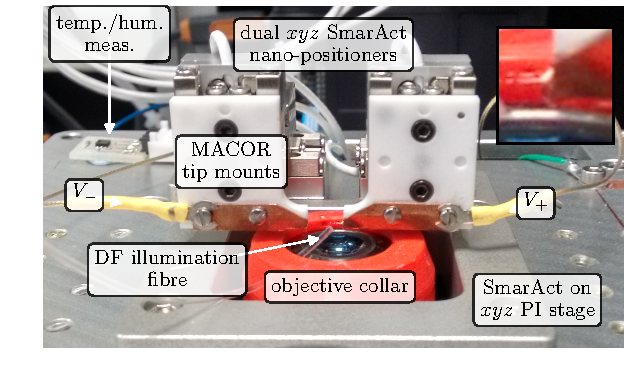
\includegraphics[width=\textwidth, clip=true, trim=20 10 0 0]{figures/tip_mount_design}
	\caption[Design of the dual tip mount stage and dark-field illumination mechanics]{\textbf{Design of the dual tip mount stage and dark-field illumination mechanics}. Each nanopositioner with tip mount clamp is connected to an external electronic circuit. A 3D-printed, plastic collar is attached to the objective, holding a \SI{1}{mm} diameter optical fibre for dark-field side-illumination of tips. A temperature and humidity sensor is attached to the back of the plate for environmental monitoring when the chamber is sealed.}
	\label{fig:tip_mount_design}
\end{subfigure}
\caption[Design of the dual tip microscope stage]{\textbf{Design of the dual tip microscope stage.}}
\end{figure}

% Sample mounts
The typical experiment sample setup is show in \figurename~\ref{fig:tip_mount_design}. Samples are mounted onto either of two 3-axis slip-stick translation stages with \SI{12}{mm} of travel and fine piezo control (SmarAct GmbH, SLC-1720-S w/ MCS), of which one is mounted onto a 3-axis piezo translation stage (PI GmbH, PI-733.3CD) for finer motion control. The top platform design is modular and easily removable, with alignment socket precise enough to relocate a sample to within \SI{10}{\micro\metre} after removal. Multiple adapters are used to mount different samples onto the stage. A cover slip holder is used for nanoparticle characterisation while AFM chip holders (\figurename~\ref{fig:tip_mount}) are designed to mount tips.
% Tip mounts
AFM probe mounts are made from machinable glass-ceramic (MACOR, Corning inc.) in order to prevent thermal expansion (coefficient of thermal expansion $\gls{thermal_expansion}=\SI{9.3e-6}{\per\kelvin}$, compared to $\alpha_{T,\mathrm{aluminium}}=\SI{23.1e-6}{\per\kelvin}$ and $\alpha_{T, \mathrm{titanium}}=\SI{8.6e-6}{\per\kelvin}$ \cite{haynes2013crc}) and to electrically insulate the mounts from the nanopositioners. The copper clamps holding the AFM probes are contacted to enable sample biasing with an applied voltage and to measure the current between two tips. Optical reference substrates (\SI{0.3}{mm} Au- and Pt-coated AFM chips) for measuring the spectral content of the illumination are attached underneath the piezo-mounted stage for {\color{red}in-situ} referencing.

% Chamber plumbing
The experimental chamber is sealed to control the gas environment (switchable between air bubbled through water and nitrogen to control humidity) and acts as a faraday cage to reduce EMI incident on the sample. The chamber is equipped with a low pressure one-way value and a needle valve to control the gas flow. Silencers are attached to the gas inlets with a foam surround to prevent air currents. The presence of a sealed chamber is enough to stabilise the sample against external air currents and helps to maintain a constant thermal equilibrium around the sample.
% Top inspection microscope
A low magnification simple microscope, constructed from a disassembled webcam CCD, is attached to the roof of the chamber to aid the alignment of samples to the objective focus. Metal contacts connect the roof to the grounded base, transforming the chamber into a EMI-shielded Faraday cage.
% Optical windows
Optical windows on the sides of the chamber are used to insert secondary lasers perpendicular to the objective axis, used primarily with the AFM module. They also allow for external monitoring of the stage positions from the side.

\FloatBarrier
\end{document}